%% Customizations over the file abtex2-modelo-trabalho-academico.tex, v-1.7.1
%% to employ the style dc-uel.cls that defines the template for documents
%% of the Departamento de Computação of the Universidade Estadual de Londrina.
%%
%% Informações sobre o arquivo original:
%% abtex2-modelo-trabalho-academico.tex, v-1.7.1 laurocesar
%% Copyright 2012-2013 by abnTeX2 group at http://abntex2.googlecode.com/ 
%%
%% This work may be distributed and/or modified under the
%% conditions of the LaTeX Project Public License, either version 1.3
%% of this license or (at your option) any later version.
%% The latest version of this license is in
%%   http://www.latex-project.org/lppl.txt
%% and version 1.3 or later is part of all distributions of LaTeX
%% version 2005/12/01 or later.
%%
%% This work has the LPPL maintenance status `maintained'.
%% 
%% The Current Maintainer of this work is Daniel dos Santos Kaster, 
%% dskaster@uel.br
%%
%% This work requires the original files
%% abntex2-modelo-include-comandos, abntex2-modelo-references.bib
%% and abntex2-modelo-img-grafico.pdf
%%

% ------------------------------------------------------------------------
% ------------------------------------------------------------------------
% abnTeX2: Modelo de Trabalho Academico (tese de doutorado, dissertacao de
% mestrado e trabalhos monograficos em geral) em conformidade com 
% ABNT NBR 14724:2011: Informacao e documentacao - Trabalhos academicos -
% Apresentacao
% ------------------------------------------------------------------------
% ------------------------------------------------------------------------

\documentclass[
	% -- opções da classe memoir --
	12pt,				% tamanho da fonte
	openright,			% capítulos começam em pág ímpar (insere página vazia caso preciso)
	oneside,			% twoside para impressão em verso e anverso. Oposto a oneside
	a4paper,			% tamanho do papel. 
	% -- opções da classe dc-uel --
	tccpreliminar,			% tipo do trabalho (opções: tcc, tccpreliminar, dissertacao, qualificacaoms)
					% - tcc (Versão para a Banca do TCC ou Versão Final do TCC)
					% - tccpreliminar (Versão Preliminar do TCC)
					% - dissertação (Versão para a Banca da Dissertação ou Versão Final/Revisada da Dissertação)
					% - qualificacaoms (Qualificação de Mestrado)
	]{ABNT-DC-UEL}


% ---
% PACOTES
% ---

% ---
% Pacotes fundamentais 
% ---
\usepackage[T1]{fontenc}		% Selecao de codigos de fonte.
\usepackage[utf8]{inputenc}		% Codificacao do documento (conversão automática dos acentos)
\usepackage{graphicx}			% Inclusão de gráficos
\usepackage{pdfpages}			% Inclusão de (páginas de) arquivos PDF no documento
% ---
		
% ---
% Pacotes adicionais, usados apenas no âmbito do Modelo Canônico do abnteX2
% ---
\usepackage{lipsum}				% para geração de dummy text
% ---

% ---
% Informações de dados para CAPA, FOLHA DE ROSTO e outros elementos
% ---
\titulo{Aplicações do Aprendizado de Máquina na geração de código \textit{spill}}
\tituloingles{Machine Learning applications in spill code generation}
\palavraschave{Compiladores. Aprendizado de Máquina. Código spill. Alocação de registradores. Otimização}
\palavraschaveingles{Compilers. Machine Learning. Spill code. Register allocation. Optimization.}
\autor{Matheus Pires Vila Real}
\citacaoautor{VILA REAL, M.}
\data{2023}

\diadefesa{24 de novembro}
\orientador{Prof. Dr. Wesley Attrot} % É membro nato e presidente da Banca Examinadora
% \coorientador{Prof(a). Dr(a). Nome do(a) Coorientador(a)} % Pode ou não ser membro da Banca; se for, deve ser incluído como membro a seguir
\membrobancadois{Prof. Dr. Segundo Membro da Banca}
\instmembrobancadois{Universidade Estadual de Londrina}
\membrobancatres{Prof. Dr. Terceiro Membro da Banca}
\instmembrobancatres{Universidade Estadual de Londrina}

% ---
% compila o indice
% ---
\makeindex
% ---

% ----
% Início do documento
% ----
\begin{document}

% Retira espaço extra obsoleto entre as frases.
\frenchspacing 

% ----------------------------------------------------------
% ELEMENTOS PRÉ-TEXTUAIS
% ----------------------------------------------------------
% \pretextual

% ---
% Capa (elemento obrigatório)
% ---
\imprimircapa
% ---

% ---
% Folha de rosto (elemento obrigatório)
% (o * indica que haverá a ficha bibliográfica)
% ---
\imprimirfolhaderosto*
% ---

% ---
% Ficha bibliografica (elemento obrigatório para versões finais de TCC e dissertação)
% ---

% Isto é um exemplo de Ficha Catalográfica, ou ``Dados internacionais de
% catalogação-na-publicação''. Você poderá utilizar o site da biblioteca para 
% gerar esta ficha através do link: http://www.uel.br/bc/ficha/. Quando estiver
% com o documento, salve-o como PDF no diretório do seu projeto e substitua todo
% o conteúdo de implementação deste arquivo pelo comando abaixo:
%
\begin{fichacatalografica}
    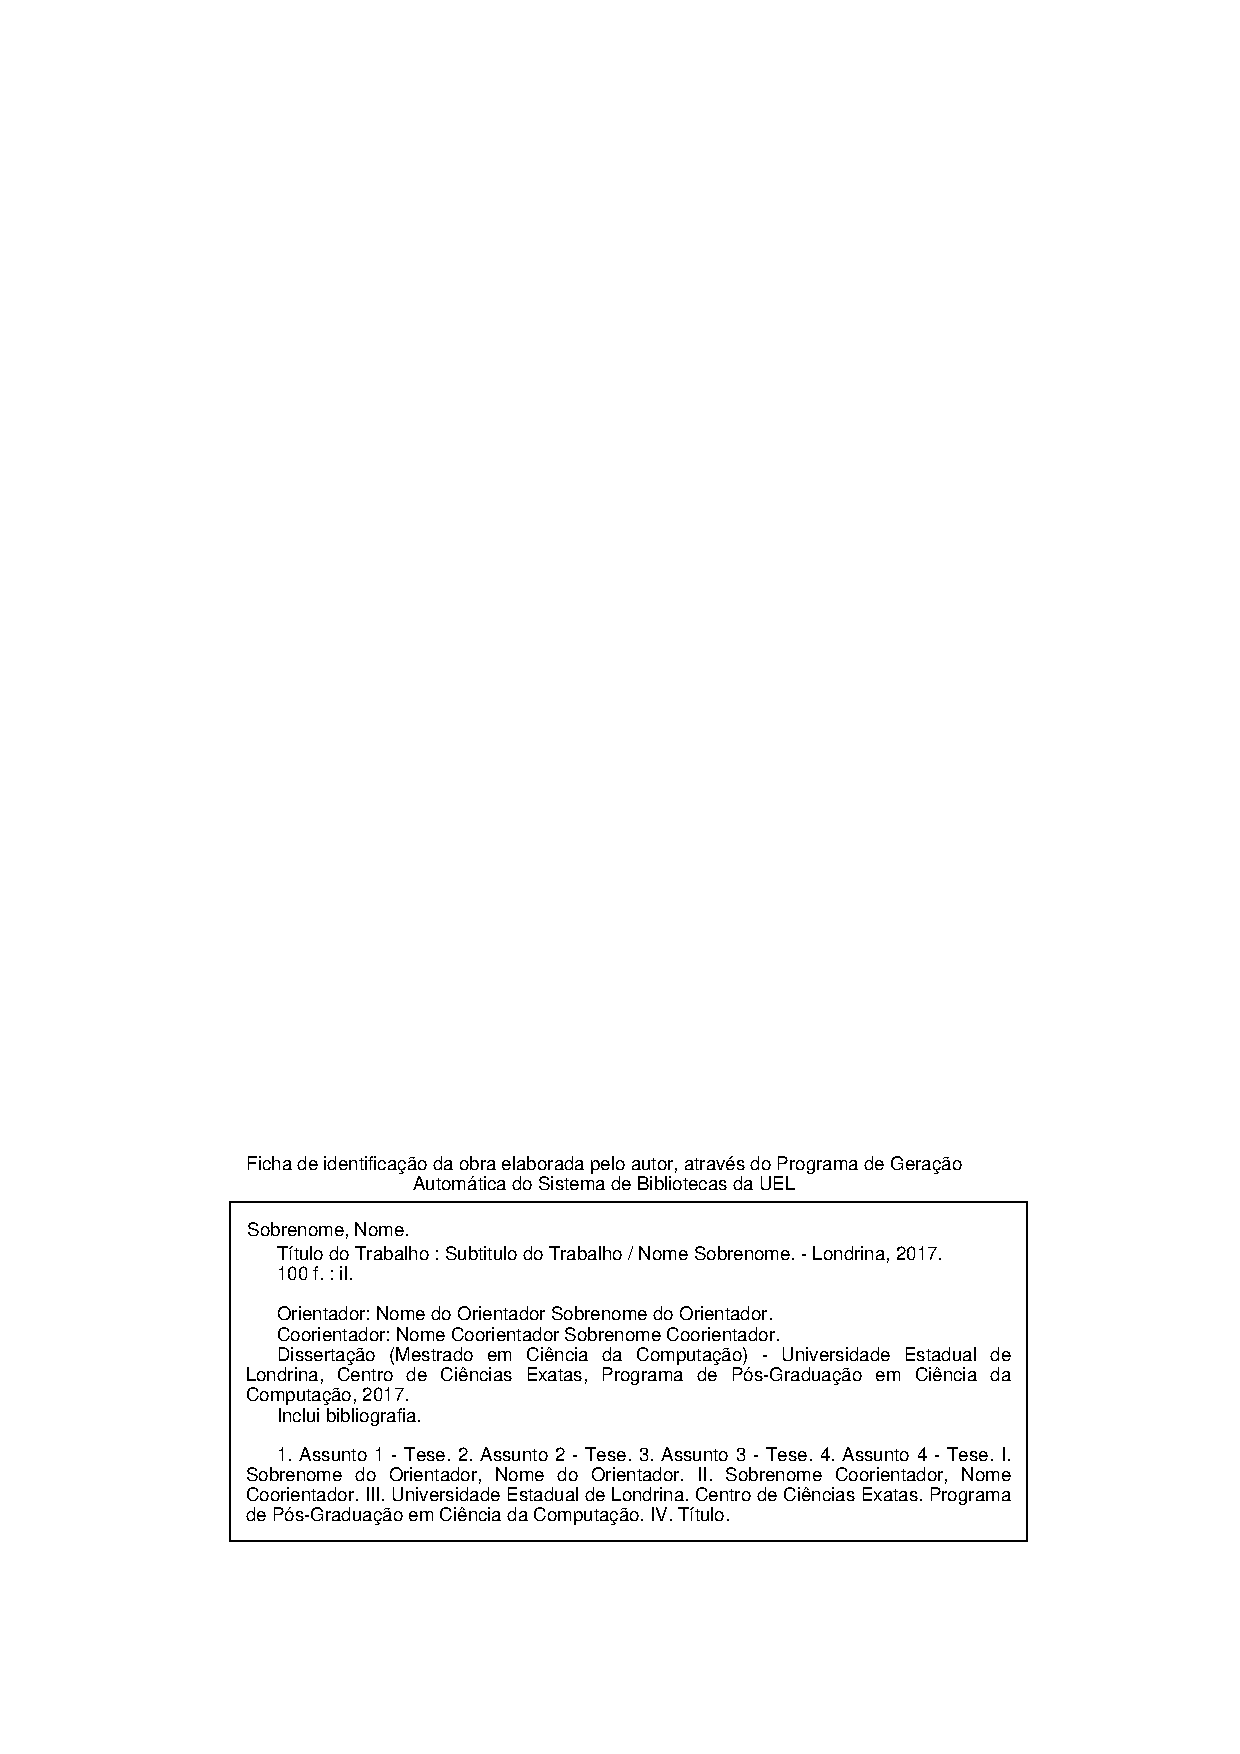
\includepdf{ficha_catalografica.pdf}
\end{fichacatalografica}


% ---

% ---
% Folha de aprovação (elemento obrigatório) ==> deve ser omitida no caso de tccpreliminar
% ---

% Isto é um exemplo de Folha de aprovação, elemento obrigatório da NBR
% 14724/2011 (seção 4.2.1.3). Você pode utilizar este modelo até a aprovação
% do trabalho. Após isso, substitua todo o conteúdo deste arquivo por uma
% imagem da página assinada pela banca com o comando abaixo:
%
% \includepdf{folhadeaprovacao_final.pdf}
\imprimirfolhadeaprovacao
% ---

% ---
% Dedicatória (elemento opcional)
% ---
\begin{dedicatoria}
  \vspace*{\fill}
  \hspace{.4\textwidth}
  \begin{minipage}{.5\textwidth}
    \begin{flushright}
      \textit{Este trabalho é dedicado às crianças adultas que, quando pequenas, sonharam em se tornar cientistas.}
    \end{flushright}  
  \end{minipage}
\end{dedicatoria}
% ---

% ---
% Agradecimentos (elemento opcional, mas fortemente recomendado)
% ---
\begin{agradecimentos}
Os agradecimentos principais são direcionados à Gerald Weber, Miguel Frasson,
Leslie H. Watter, Bruno Parente Lima, Flávio de Vasconcellos Corrêa, Otavio Real
Salvador, Renato Machnievscz\footnote{Os nomes dos integrantes do primeiro
projeto abn\TeX\ foram extraídos de
\url{http://codigolivre.org.br/projects/abntex/}} e todos aqueles que
contribuíram para que a produção de trabalhos acadêmicos conforme
as normas ABNT com \LaTeX\ fosse possível.

Agradecimentos especiais são direcionados ao Centro de Pesquisa em Arquitetura
da Informação\footnote{\url{http://www.cpai.unb.br/}} da Universidade de
Brasília (CPAI), ao grupo de usuários
\emph{latex-br}\footnote{\url{http://groups.google.com/group/latex-br}} e aos
novos voluntários do grupo
\emph{\abnTeX}\footnote{\url{http://groups.google.com/group/abntex2} e
\url{http://abntex2.googlecode.com/}}~que contribuíram e que ainda
contribuirão para a evolução do \abnTeX.

\end{agradecimentos}
% ---

% ---
% Epígrafe (elemento opcional)
% ---
\begin{epigrafe}
  \vspace*{\fill}
  \hspace{.4\textwidth}
  \begin{minipage}{.5\textwidth}   
    \begin{flushright}
	\textit{
    ``Não vos amoldeis às estruturas deste mundo,
      mas transformai-vos pela renovação da mente,
      a fim de distinguir qual é a vontade de Deus:
      o que é bom, o que Lhe é agradável, o que é perfeito.\\
      (Bíblia Sagrada, Romanos 12, 2))}
    \end{flushright}
  \end{minipage}
\end{epigrafe}
% ---

% ---
% RESUMOS
% ---

% ---
% Resumo em Português (elemento obrigatório)
% ---
\begin{resumo}
A alocação de registradores é uma das otimizações de código mais significativas do processo de compilação de um programa. Mas, devido à natureza dos algoritmos empregados nas implementações tradicionais, ela caracteriza-se como um prolema NP-completo, o qual é difícil de se resolver de maneira ótima. Nesse contexto, ao longo dos anos foram sendo propostas heurísticas e ajustes visando tornar as técnicas de geração de código \textit{spill} mais precisas e menos custosas. Com o crescimento da relevância do aprendizado de máquina (\textit{machine learning}) --- área da inteligência artificial, que engloba o desenvolvimento de modelos complexos de categorização e predição treinados de maneira algorítmica --- surge a perspectiva de integração de ambas as áreas. Isto posto, este trabalho se propõe a vislumbrar o estado da arte da aplicação do aprendizado de máquina na alocação de registradores e investigar as possibilidades práticas de implementação de alocadores utilizando modelos treinados por \textit{machine learning}.
\end{resumo}
% ---

% ---
% Resumo em Inglês (elemento obrigatório)
% ---
% O ambiente Abstract (com A maiúsculo) é definido no estilo dc-uel
\begin{Abstract}
Register allocation is highlighted as one of the key code optimizations throughout a program's compilation process. It is, however, a NP-complete problem, due to the nature of the traditional implementations, which are unable to obtain optimal solutions in reasonable time. In this context, several heuristics and adjustments have been proposed over the course of the years in order to improve the precision and the speed of register allocators. Machine learning, in the other hand, is a field of artificial intelligence encompassing the development of complex classification and prediction models which are trained in an algorithmic way, that grew in relevance and became widely researched recently. Therefore, efforts to apply machine learning techniques to register allocation, aiming to improve spill code generation, arose. This work is intended to examine the current state-of-the-art of the integration of both fields and investigate the implementation possiblities of register allocators that widely employ machine learning models in their inner workings.
\end{Abstract}
% ---

% ---
% Lista de ilustrações (elemento opcional, mas fortemente recomendado)
% ---
\pdfbookmark[0]{\listfigurename}{lof}
\listoffigures*
\cleardoublepage
% ---

% ---
% Lista de tabelas (elemento opcional, mas fortemente recomendado)
% ---
\pdfbookmark[0]{\listtablename}{lot}
\listoftables*
\cleardoublepage
% ---

% ---
% Lista de abreviaturas e siglas (elemento opcional)
% ---
\begin{siglas}
  % \item[ABNT] Associação Brasileira de Normas Técnicas
  % \item[BNDES] Banco Nacional de Desenvolvimento Econômico e Social
  % \item[IBGE] Instituto Nacional de Geografia e Estatística
  % \item[IBICT] Instituto Brasileiro de Informação em Ciência e Tecnologia
  % \item[NBR] Norma Brasileira
  \item[CPU] \textit{Central Processing Unit}
\end{siglas}
% ---

% ---
% Lista de símbolos (elemento opcional)
% ---
% \begin{simbolos}
%   \item[$ \Gamma $] Letra grega Gama
%   \item[$ \Lambda $] Lambda
%   \item[$ \zeta $] Letra grega minúscula zeta
%   \item[$ \in $] Pertence
% \end{simbolos}
% ---

% ---
% Sumario (elemento obrigatório)
% ---
\pdfbookmark[0]{\contentsname}{toc}
\tableofcontents*
\cleardoublepage
% ---



% ----------------------------------------------------------
% ELEMENTOS TEXTUAIS
% ----------------------------------------------------------
\textual
\pagestyle{dc-uel-header} % Configura cabeçalho para apresentar apenas números de página


% ----------------------------------------------------------
% Introdução
% ----------------------------------------------------------
\chapter{Introdução}
Os compiladores constituem uma das classes de programa mais importantes na Ciência da Computação, cuja principal função é a tradução de código-fonte de uma linguagem de programação para outra. Usualmente, esse processo é empregado para transformar código de alto nível em linguagem de máquina de baixo nível, executável diretamente pelo processador de determinada arquitetura-alvo. \cite{aho:07}.

Para atingir esse objetivo, o compilador deve submeter o programa original a uma série de análises --- léxica, sintática e semântica --- a fim de criar uma representação lógica de sua estrutura e prosseguir com a geração de código. Entre essas duas etapas, é desejável efetuar algumas otimizações a fim de tornar o binário final mais eficiente do ponto de vista de execução e mais coerente com as especificidades da arquitetura-alvo \cite{muchnick:97}.

Dentre as etapas de otimização, destaca-se a alocação de registradores, onde o compilador deve distribuir os registradores para as variáveis utilizadas ao longo do fluxo de execução do programa. Os registradores são componentes microarquiteturais diretamente disponíveis ao processador, e caracterizam-se como as unidades de memória de mais rápido acesso \cite{mittal:16}. Contudo, sendo eles um recurso finito, surge a possibilidade de não haverem registradores o suficiente para comportar todos os valores e resultados intermediários em memória de uma única vez \cite{aho:07}.

Nesses casos, há a necessidade de se mapear algumas variáveis para a memória principal, e o compilador deve então introduzir no código instruções de acesso à memória para salvar e recuperar os valores lá armazenados. Essas instruções são denominadas código \textit{spill}, ou \textit{spill code} \cite{briggs:92}. Um esquema de alocação ideal deve buscar minimizar o tráfego entre a memória principal e a CPU, visto que essas operações, em comparação com o acesso a registradores, são significativamente mais lentas e dispendiosas do ponto de vista energético. As operações em memória representam de 50\% a 75\% dos gastos de energia de um sistema computacional \cite{verma:06}, e um alocador sofisticado pode proporcionar uma melhora de até 250\% no tempo de execução de um programa comparado a um alocador simples \cite{pereira:08}.

A abordagem tradicional emprega a coloração de grafo como abstração para representar o processo de atribuição dos registradores físicos para as variáveis virtuais. Nesse modelo, os valores em memória --- chamados de registradores virtuais da representação intermediária do código --- são expressos como os nós de um grafo a ser colorido; as arestas representam as relações de interferência entre os registradores virtuais, isto é, a presença de intersecções entre o tempo de vida dos valores em memória, enquanto que a coloração em si seria o processo de encontrar registradores físicos disponíveis para cada variável \cite{chaitin:81}.

Contudo, produzir uma alocação eficiente não é uma tarefa trivial. A coloração de grafos é um problema NP-completo, isto é, não há algoritmos determinísticos que a resolvam em tempo polinomial \cite{karp:72}, e descobrir a mera quantidade de cores necessárias para colorir um grafo é um problema difícil \cite{garey:76}. Ademais, uma implementação ingênua pode introduzir \textit{spill code} desnecessário ao longo de todo o tempo de vida de um registrador virtual \cite{bergner:97}, ou realizar escolhas ruins sobre quais variáveis enviar para a memória principal, ao eleger valores frequentemente utilizados no código e que exigirão uma grande quantidade de acessos ou escritas à memória \cite{bernstein:89}.

Ao longo dos anos, soluções para se contornar essas dificuldades foram propostas: ajustes no algoritmo original, visando tornar a introdução de \textit{spill code} mais precisa nos pontos de interferência necessários \cite{chaitin:82, briggs:92, briggs2:92, cooper:98}, e a utilização de heurísticas para cálculo de custo de \textit{spill}, visando melhorar a qualidade das escolhas de quais variáveis mapear para a memória principal. Infelizmente, as heurísticas dependem de uma boa quantidade de ajustes para propiciar um desempenho adequado. O desenvolvimento de um conjunto de heurísticas para uma arquitetura-alvo específica ainda é feito através de tentativa e erro, e o ajuste fino das funções prioritárias é um processo tedioso \cite{amarasinghe:03}.

O aprendizado de máquina (\textit{machine learning}), por sua vez, é uma área da inteligência artificial que abrange o desenvolvimento de modelos e agentes inteligentes treinados de maneira algorítmica. Eles realizam tarefas de predição e classificação probabilísticas a partir de parâmetros de entrada, e são calibrados após sucessivas iterações de treinamento, onde os resultados de saída são confrontados com um conjunto de dados previamente conhecidos sobre o problema, de modo a se calcular um erro e ajustar os parâmetros internos do modelo para minimizá-lo \cite{sharma:21}.

Nas últimas décadas, o aprendizado de máquina e a inteligência artificial como um todo vem avançando consideravelmente, graças ao crescimento do poder computacional das máquinas e conforme cada vez mais dados são gerados e coletados \cite{alpaydin:20}. Esse cenário expande os horizontes para a integração de ambas as áreas, que almeja o desenvolvimento de melhores heurísticas e métodos para otimizar a alocação de registradores empregando técnicas de aprendizado de máquina. Trabalhos vêm sendo publicados explorando a interdisciplinaridade de ambas as áreas e trazendo resultados animadores ou, ao menos, de interesse, como é o caso das pesquisas de Amarasinghe \textit{et al.}, Das \textit{et al.} e VenkataKeerthy \textit{et al.} \cite{amarasinghe:03, das:20, venkatakeerthy:23}.

Este trabalho se propõe a investigar a aplicação das técnicas de aprendizado de máquina na alocação de registradores, particularmente sua utilidade na geração de código \textit{spill}. Ele irá contemplar o estado da arte da alocação de registradores e, apoiado no conhecimento acadêmico sobre a área, serão propostos métodos de alocação e heurísticas que utilizam \textit{machine learning}.

% ----------------------------------------------------------
% PARTE
% ----------------------------------------------------------
% A organização dos capítulos em partes só é recomendada caso o texto seja muito extenso
% Não é comum dividir o trabalho em partes em TCCs e dissertações de mestrado

%\part{Preparação da pesquisa}

% ----------------------------------------------------------
% Capitulo com exemplos de comandos inseridos de arquivo externo 
% ----------------------------------------------------------

% %% abtex2-modelo-include-comandos.tex, v-1.7.1 laurocesar
%% Copyright 2012-2013 by abnTeX2 group at http://abntex2.googlecode.com/ 
%%
%% This work may be distributed and/or modified under the
%% conditions of the LaTeX Project Public License, either version 1.3
%% of this license or (at your option) any later version.
%% The latest version of this license is in
%%   http://www.latex-project.org/lppl.txt
%% and version 1.3 or later is part of all distributions of LaTeX
%% version 2005/12/01 or later.
%%
%% This work has the LPPL maintenance status `maintained'.
%% 
%% The Current Maintainer of this work is the abnTeX2 team, led
%% by Lauro César Araujo. Further information are available on 
%% http://abntex2.googlecode.com/
%%
%% This work consists of the files abntex2-modelo-include-comandos.tex
%%

% ---
% Este capítulo, utilizado por diferentes exemplos do abnTeX2, ilustra o uso de
% comandos do abnTeX2 e de LaTeX.
% ---
 
\chapter{Resultados de comandos}\label{cap_exemplos}

\chapterprecis{Isto é uma sinopse de capítulo. A ABNT não traz nenhuma
normatização a respeito desse tipo de resumo, que é mais comum em romances 
e livros técnicos.}\index{sinopse de capítulo}

% ---
\section{Codificação dos arquivos: UTF8}
% ---

A codificação de todos os arquivos do \abnTeX2 é \texttt{UTF8}. É necessário que
você utilize a mesma codificação nos documentos que escrever, inclusive nos
arquivos de base bibliográficas |.bib|.

% ---
\section{Citações diretas}
\label{sec-citacao}
% ---

\index{citações!diretas}Utilize o ambiente \texttt{citacao} para incluir
citações diretas com mais de três linhas:

\begin{citacao}
As citações diretas, no texto, com mais de três linhas, devem ser
destacadas com recuo de 4 cm da margem esquerda, com letra menor que a do texto
utilizado e sem as aspas. No caso de documentos datilografados, deve-se
observar apenas o recuo \cite[5.3]{NBR10520:2002}.
\end{citacao}

Use o ambiente assim:

\begin{verbatim}
\begin{citacao}
As citações diretas, no texto, com mais de três linhas [...] deve-se observar
apenas o recuo \cite[5.3]{NBR10520:2002}.
\end{citacao}
\end{verbatim}

O ambiente \texttt{citacao} pode receber como parâmetro opcional um nome de
idioma previamente carregado nas opções da classe (\autoref{sec-hifenizacao}). Nesse
caso, o texto da citação é automaticamente escrito em itálico e a hifenização é
ajustada para o idioma selecionado na opção do ambiente. Por exemplo:

\begin{verbatim}
\begin{citacao}[english]
Text in English language in italic with correct hyphenation.
\end{citacao}
\end{verbatim}

Tem como resultado:

\begin{citacao}[english]
Text in English language in italic with correct hyphenation.
\end{citacao}

\index{citações!simples}Citações simples, com até três linhas, devem ser
incluídas com aspas. Observe que em \LaTeX as aspas iniciais são diferentes das
finais: ``Amor é fogo que arde sem se ver''.

% ---
\section{Notas de rodapé}
% ---

As notas de rodapé são detalhadas pela NBR 14724:2011 na seção 5.2.1\footnote{As
notas devem ser digitadas ou datilografadas dentro das margens, ficando
separadas do texto por um espaço simples de entre as linhas e por filete de 5
cm, a partir da margem esquerda. Devem ser alinhadas, a partir da segunda linha
da mesma nota, abaixo da primeira letra da primeira palavra, de forma a destacar
o expoente, sem espaço entre elas e com fonte menor
\citeonline[5.2.1]{NBR14724:2011}.}\footnote{Caso uma série de notas sejam
criadas sequencialmente, o \abnTeX\ instrui o \LaTeX\ para que uma vírgula seja
colocada após cada número do expoente que indica a nota de rodapé no corpo do
texto.}\footnote{Verifique se os números do expoente possuem uma vírgula para
dividi-los no corpo do texto.}. 


% ---
\section{Tabelas}
% ---

\index{tabelas}A \autoref{tab-nivinv} é um exemplo de tabela construída em
\LaTeX.

\begin{table}[htb]
\footnotesize
\caption[Níveis de investigação]{Níveis de investigação. (Fonte: \citeonline{van86})}
\label{tab-nivinv}
\begin{tabular}{p{2.6cm}|p{6.0cm}|p{2.25cm}|p{3.40cm}}
  %\hline
   \textbf{Nível de Investigação} & \textbf{Insumos}  & \textbf{Sistemas de Investigação}  & \textbf{Produtos}  \\
    \hline
    Meta-nível & Filosofia\index{filosofia} da Ciência  & Epistemologia &
    Paradigma  \\
    \hline
    Nível do objeto & Paradigmas do metanível e evidências do nível inferior &
    Ciência  & Teorias e modelos \\
    \hline
    Nível inferior & Modelos e métodos do nível do objeto e problemas do nível inferior & Prática & Solução de problemas  \\
   % \hline
\end{tabular}
\end{table}

% ---
\section{Figuras}
% ---

\index{figuras}Figuras podem ser criadas diretamente em \LaTeX,
como o exemplo da \autoref{fig_circulo}.

\begin{figure}[htb]
	\begin{center}
	    \setlength{\unitlength}{5cm}
		\begin{picture}(1,1)
		\put(0,0){\line(0,1){1}}
		\put(0,0){\line(1,0){1}}
		\put(0,0){\line(1,1){1}}
		\put(0,0){\line(1,2){.5}}
		\put(0,0){\line(1,3){.3333}}
		\put(0,0){\line(1,4){.25}}
		\put(0,0){\line(1,5){.2}}
		\put(0,0){\line(1,6){.1667}}
		\put(0,0){\line(2,1){1}}
		\put(0,0){\line(2,3){.6667}}
		\put(0,0){\line(2,5){.4}}
		\put(0,0){\line(3,1){1}}
		\put(0,0){\line(3,2){1}}
		\put(0,0){\line(3,4){.75}}
		\put(0,0){\line(3,5){.6}}
		\put(0,0){\line(4,1){1}}
		\put(0,0){\line(4,3){1}}
		\put(0,0){\line(4,5){.8}}
		\put(0,0){\line(5,1){1}}
		\put(0,0){\line(5,2){1}}
		\put(0,0){\line(5,3){1}}
		\put(0,0){\line(5,4){1}}
		\put(0,0){\line(5,6){.8333}}
		\put(0,0){\line(6,1){1}}
		\put(0,0){\line(6,5){1}}
		\end{picture}
	\end{center}
	\caption{\label{fig_circulo}A delimitação do espaço}
\end{figure}

Ou então figuras podem ser incorporadas de arquivos externos, como é o caso da
\autoref{fig_grafico}. Se a figura que ser incluída se tratar de um diagrama, um
gráfico ou uma ilustração que você mesmo produza, priorize o uso de imagens
vetoriais no formato PDF. Com isso, o tamanho do arquivo final do trabalho será
menor, e as imagens terão uma apresentação melhor, principalmente quando
impressas, uma vez que imagens vetorias são perfeitamente escaláveis para
qualquer dimensão. Nesse caso, se for utilizar o Microsoft Excel para produzir
gráficos, ou o Microsoft Word para produzir ilustrações, exporte-os como PDF e
os incorpore ao documento conforme o exemplo abaixo. No entanto, para manter a
coerência no uso de software livre (já que você está usando \LaTeX e \abnTeX),
teste a ferramenta \textsf{InkScape}\index{InkScape}
(\url{http://inkscape.org/}). Ela é uma excelente opção de código-livre para
produzir ilustrações vetoriais, similar ao CorelDraw\index{CorelDraw} ou ao Adobe
Illustrator\index{Adobe Illustrator}. De todo modo, caso não seja possível
utilizar arquivos de imagens como PDF, utilize qualquer outro formato, como
JPEG, GIF, BMP, etc. Nesse caso, você pode tentar aprimorar as imagens
incorporadas com o software livre \textsf{Gimp}\index{Gimp}
(\url{http://www.gimp.org/}). Ele é uma alternativa livre ao Adobe
Photoshop\index{Adobe Photoshop}.

\begin{figure}[htb]
	\begin{center}
	    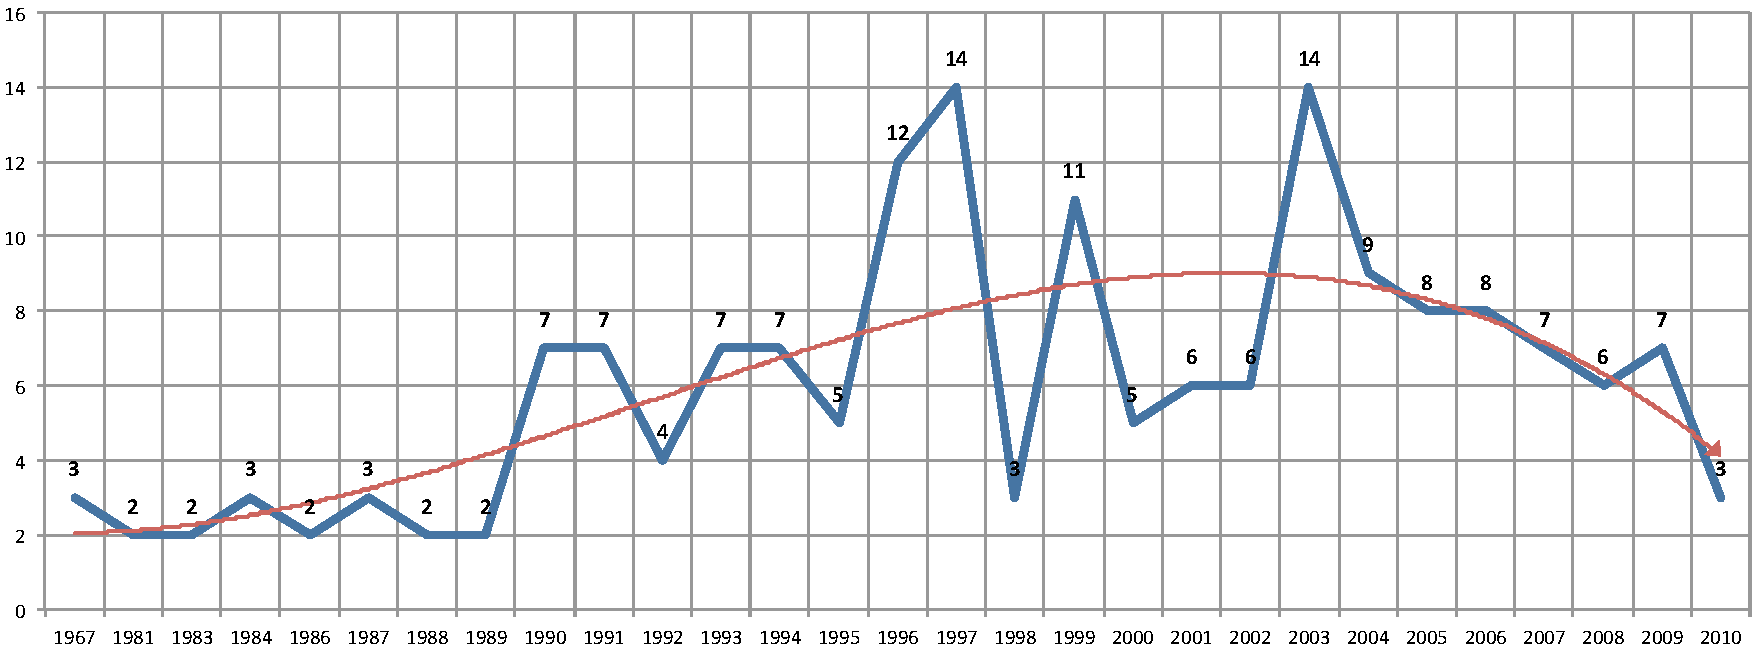
\includegraphics[scale=0.5]{abntex2-modelo-img-grafico.pdf}
	\end{center}
	\caption{\label{fig_grafico}Gráfico produzido em Excel e salvo como PDF. (Fonte: \citeonline[p. 24]{araujo2012})}
\end{figure}

% ---
\subsection{Figuras em \emph{minipages}}
% ---

\emph{Minipages} são usadas para inserir textos ou outros elementos em quadros
com tamanhos e posições controladas. Veja o exemplo da
\autoref{fig_minipage_grafico1} e da \autoref{fig_minipage_grafico2}.

\begin{figure}[htb]
 \label{teste}
 \centering
  \begin{minipage}{0.4\textwidth}
    \centering
    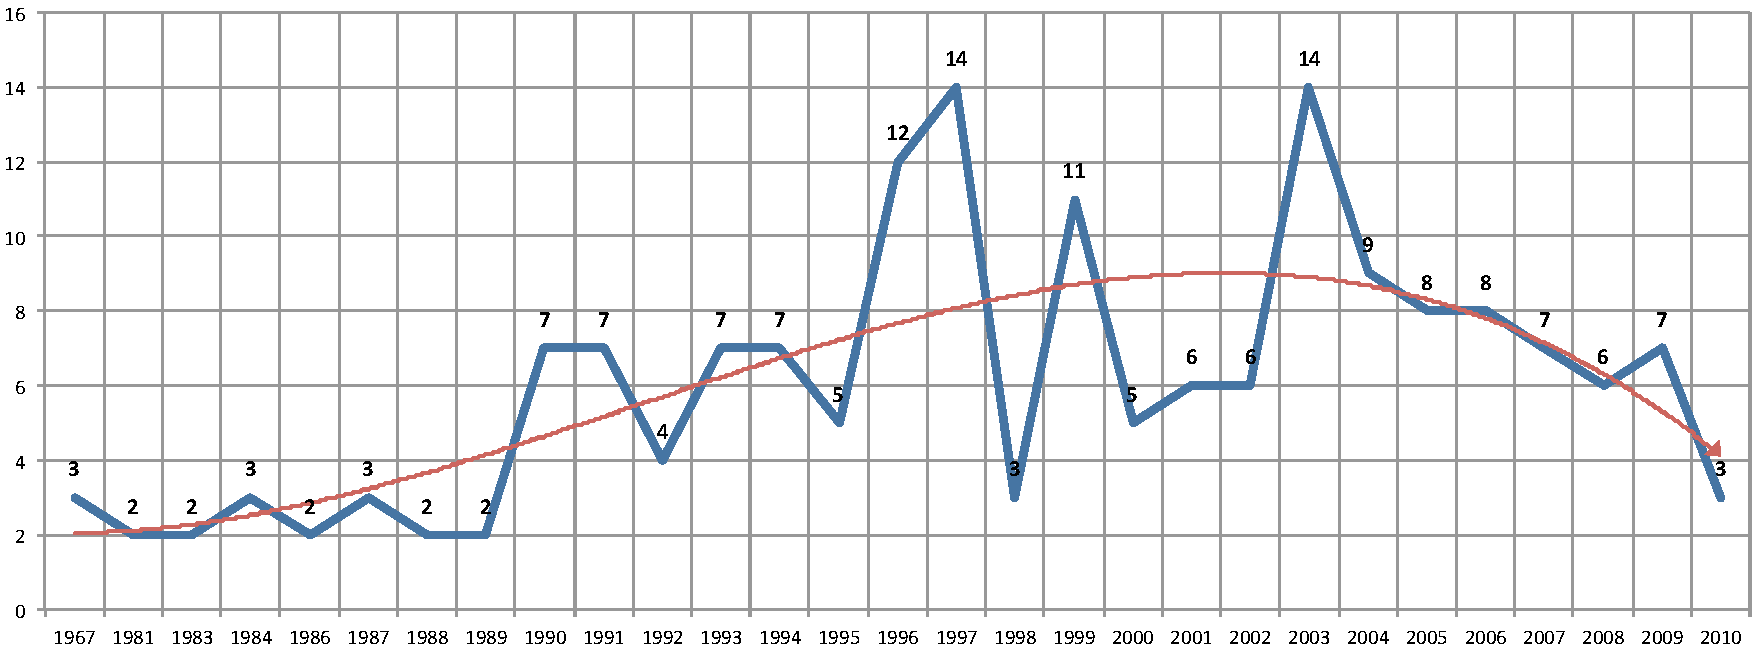
\includegraphics[scale=0.2]{abntex2-modelo-img-grafico.pdf}
    \caption{Grafico 1 da minipage. (Fonte: \citeonline[p. 24]{araujo2012})} \label{fig_minipage_grafico1}
  \end{minipage}
  \hfill
  \begin{minipage}{0.4\textwidth}
    \centering
    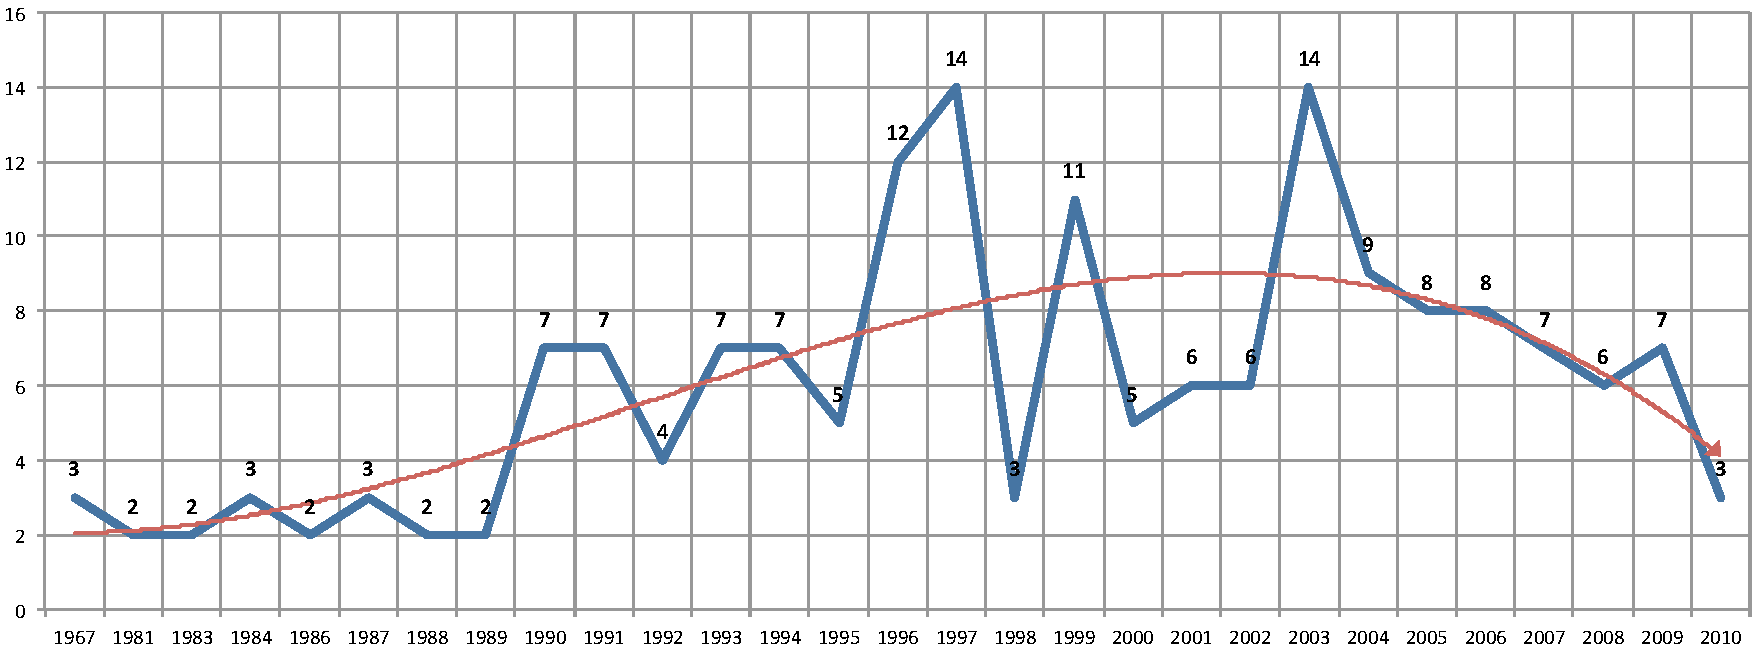
\includegraphics[scale=0.2]{abntex2-modelo-img-grafico.pdf}
    \caption{Grafico 2 da minipage. (Fonte: \citeonline[p. 24]{araujo2012})} \label{fig_minipage_grafico2}
  \end{minipage}
\end{figure}

Observe que, segundo a \citeonline[seções 4.2.1.10 e 5.8]{NBR14724:2011}, as
ilustrações devem sempre ter numeração contínua e única em todo o documento:

\begin{citacao}
Qualquer que seja o tipo de ilustração, sua identificação aparece na parte
superior, precedida da palavra designativa (desenho, esquema, fluxograma,
fotografia, gráfico, mapa, organograma, planta, quadro, retrato, figura,
imagem, entre outros), seguida de seu número de ordem de ocorrência no texto,
em algarismos arábicos, travessão e do respectivo título. Após a ilustração, na
parte inferior, indicar a fonte consultada (elemento obrigatório, mesmo que
seja produção do próprio autor), legenda, notas e outras informações
necessárias à sua compreensão (se houver). A ilustração deve ser citada no
texto e inserida o mais próximo possível do trecho a que se
refere. \cite[seções 5.8]{NBR14724:2011}
\end{citacao}

% ---
\section{Expressões matemáticas}
% ---

\index{expressões matemáticas}Use o ambiente \texttt{equation} para escrever
expressões matemáticas numeradas:

\begin{equation}
  \forall x \in X, \quad \exists \: y \leq \epsilon
\end{equation}

Escreva expressões matemáticas entre \$ e \$, como em $ \lim_{x \to \infty}
\exp(-x) = 0 $, para que fiquem na mesma linha.

Também é possível usar colchetes para indicar o início de uma expressão
matemática que não é numerada.

\[
\left|\sum_{i=1}^n a_ib_i\right|
\le
\left(\sum_{i=1}^n a_i^2\right)^{1/2}
\left(\sum_{i=1}^n b_i^2\right)^{1/2}
\]

Consulte mais informações sobre expressões matemáticas em
\url{http://code.google.com/p/abntex2/w/edit/Referencias}.

% ---
\section{Enumerações: alíneas e subalíneas}
% ---

\index{alíneas}\index{subalíneas}\index{incisos}Quando for necessário enumerar
os diversos assuntos de uma seção que não possua título, esta deve ser
subdividida em alíneas \cite[4.2]{NBR6024:2012}:

\begin{alineas}

  \item os diversos assuntos que não possuam título próprio, dentro de uma mesma
  seção, devem ser subdivididos em alíneas; 
  
  \item o texto que antecede as alíneas termina em dois pontos;
  \item as alíneas devem ser indicadas alfabeticamente, em letra minúscula,
  seguida de parêntese. Utilizam-se letras dobradas, quando esgotadas as
  letras do alfabeto;

  \item as letras indicativas das alíneas devem apresentar recuo em relação à
  margem esquerda;

  \item o texto da alínea deve começar por letra minúscula e terminar em
  ponto-e-vírgula, exceto a última alínea que termina em ponto final;

  \item o texto da alínea deve terminar em dois pontos, se houver subalínea;

  \item a segunda e as seguintes linhas do texto da alínea começa sob a
  primeira letra do texto da própria alínea;
  
  \item subalíneas \cite[4.3]{NBR6024:2012} devem ser conforme as alíneas a
  seguir:

  \begin{alineas}
     \item as subalíneas devem começar por travessão seguido de espaço;

     \item as subalíneas devem apresentar recuo em relação à alínea;

     \item o texto da subalínea deve começar por letra minúscula e terminar em
     ponto-e-vírgula. A última subalínea deve terminar em ponto final, se não
     houver alínea subsequente;

     \item a segunda e as seguintes linhas do texto da subalínea começam sob a
     primeira letra do texto da própria subalínea.
  \end{alineas}
  
  \item no \abnTeX\ estão disponíveis os ambientes \texttt{incisos} e
  \texttt{subalineas}, que em suma são o mesmo que se criar outro nível de
  \texttt{alineas}, como nos exemplos à seguir:
  
  \begin{incisos}
    \item \textit{Um novo inciso em itálico};
  \end{incisos}
  
  \item Alínea em \textbf{negrito}:
  
  \begin{subalineas}
    \item \textit{Uma subalínea em itálico};
    \item \underline{\textit{Uma subalínea em itálico e sublinhado}}; 
  \end{subalineas}
  
  \item Última alínea com \emph{ênfase}.
  
\end{alineas}

% ---
\section{Espaçamento entre parágrafos e linhas}
% ---

\index{espaçamento!dos parágrafos}O tamanho do parágrafo, espaço entre a margem
e o início da frase do parágrafo, é definido por:

\begin{verbatim}
   \setlength{\parindent}{1.3cm}
\end{verbatim}

\index{espaçamento!do primeiro parágrafo}Por padrão, não há espaçamento no
primeiro parágrafo de cada início de divisão do documento
(\autoref{sec-divisoes}). Porém, você pode definir que o primeiro parágrafo
também seja indentado, como é o caso deste documento. Para isso, apenas inclua o
pacote \textsf{indentfirst} no preâmbulo do documento:

\begin{verbatim}
   \usepackage{indentfirst}      % Indenta o primeiro parágrafo de cada seção.
\end{verbatim}

\index{espaçamento!entre os parágrafos}O espaçamento entre um parágrafo e outro
pode ser controlado por meio do comando:

\begin{verbatim}
  \setlength{\parskip}{0.2cm}  % tente também \onelineskip
\end{verbatim}

\index{espaçamento!entre as linhas}O controle do espaçamento entre linhas é
definido por:

\begin{verbatim}
  \OnehalfSpacing       % espaçamento um e meio (padrão); 
  \DoubleSpacing        % espaçamento duplo
  \SingleSpacing        % espaçamento simples	
\end{verbatim}

Para isso, também estão disponíveis os ambientes:

\begin{verbatim}
  \begin{SingleSpace} ...\end{SingleSpace}
  \begin{Spacing}{hfactori} ... \end{Spacing}
  \begin{OnehalfSpace} ... \end{OnehalfSpace}
  \begin{OnehalfSpace*} ... \end{OnehalfSpace*}
  \begin{DoubleSpace} ... \end{DoubleSpace}
  \begin{DoubleSpace*} ... \end{DoubleSpace*} 
\end{verbatim}

Para mais informações, consulte \citeonline[p. 47-52 e 135]{memoir}.

% ---
\section{Inclusão de outros arquivos}\label{sec-include}
% ---

É uma boa prática dividir o seu documento em diversos arquivos, e não
apenas escrever tudo em um único. Esse recurso foi utilizado neste
documento. Para incluir diferentes arquivos em um arquivo principal,
de modo que cada arquivo incluído fique em uma página diferente, utilize o
comando:

\begin{verbatim}
   \include{documento-a-ser-incluido}      % sem a extensão .tex
\end{verbatim}

Para incluir documentos sem quebra de páginas, utilize:

\begin{verbatim}
   \input{documento-a-ser-incluido}      % sem a extensão .tex
\end{verbatim}

% ---
\section{Compilar o documento \LaTeX}
% ---

Geralmente os editores \LaTeX, como o
TeXlipse\footnote{\url{http://texlipse.sourceforge.net/}}, o
Texmaker\footnote{\url{http://www.xm1math.net/texmaker/}}, entre outros,
compilam os documentos automaticamente, de modo que você não precisa se
preocupar com isso.

No entanto, você pode compilar os documentos \LaTeX usando os seguintes
comandos, que devem ser digitados no \emph{Prompt de Comandos} do Windows ou no
\emph{Terminal} do Mac ou do Linux:

\begin{verbatim}
   pdflatex ARQUIVO_PRINCIPAL.tex
   bibtex ARQUIVO_PRINCIPAL.aux
   makeindex ARQUIVO_PRINCIPAL.idx 
   makeindex ARQUIVO_PRINCIPAL.nlo -s nomencl.ist -o ARQUIVO_PRINCIPAL.nls
   pdflatex ARQUIVO_PRINCIPAL.tex
   pdflatex ARQUIVO_PRINCIPAL.tex
\end{verbatim}

% ---
\section{Remissões internas}
% ---

Ao nomear a \autoref{tab-nivinv} e a \autoref{fig_circulo}, apresentamos um
exemplo de remissão interna, que também pode ser feita quando indicamos o
\autoref{cap_exemplos}, que tem o nome \emph{\nameref{cap_exemplos}}. O número
do capítulo indicado é \ref{cap_exemplos}, que se inicia à
\autopageref{cap_exemplos}\footnote{O número da página de uma remissão pode ser
obtida também assim:
\pageref{cap_exemplos}.}.
Veja a \autoref{sec-divisoes} para outros exemplos de remissões internas entre
seções, subseções e subsubseções.

O código usado para produzir o texto desta seção é:

\begin{verbatim}
Ao nomear a \autoref{tab-nivinv} e a \autoref{fig_circulo}, apresentamos um
exemplo de remissão interna, que também pode ser feita quando indicamos o
\autoref{cap_exemplos}, que tem o nome \emph{\nameref{cap_exemplos}}. O número
do capítulo indicado é \ref{cap_exemplos}, que se inicia à
\autopageref{cap_exemplos}\footnote{O número da página de uma remissão pode ser
obtida também assim:
\pageref{cap_exemplos}.}.
Veja a \autoref{sec-divisoes} para outros exemplos de remissões internas entre
seções, subseções e subsubseções.
\end{verbatim}

% ---
\section{Divisões do documento: seção}\label{sec-divisoes}
% ---

Esta seção testa o uso de divisões de documentos. Esta é a
\autoref{sec-divisoes}. Veja a \autoref{sec-divisoes-subsection}.

\subsection{Divisões do documento: subseção}\label{sec-divisoes-subsection}

Isto é uma subseção. Veja a \autoref{sec-divisoes-subsubsection}, que é uma
\texttt{subsubsection} do \LaTeX, mas é impressa chamada de ``subseção'' porque
no Português não temos a palavra ``subsubseção''.

\subsubsection{Divisões do documento: subsubseção}
\label{sec-divisoes-subsubsection}

Isto é uma subsubseção.

\subsubsection{Divisões do documento: subsubseção}

Isto é outra subsubseção.

\subsection{Divisões do documento: subseção}\label{sec-exemplo-subsec}

Isto é uma subseção.

\subsubsection{Divisões do documento: subsubseção}

Isto é mais uma subsubseção da \autoref{sec-exemplo-subsec}.


\paragraph{Isto é um parágrafo rotulado}\label{sec-exemplo-paragrafo}

Este é um parágrafo na \autoref{sec-exemplo-paragrafo}. 

\paragraph{Isto é outro parágrafo rotulado}\label{sec-exemplo-paragrafo-outro}

Este é outro parágrafo na \autoref{sec-exemplo-paragrafo-outro}. 



% ---
\section{Este é um exemplo de nome de seção longo. Ele deve estar
alinhado à esquerda e a segunda e demais linhas devem iniciar logo abaixo da
primeira palavra da primeira linha}
% ---

Isso atende à norma \citeonline[seções de 5.2.2 a 5.2.4]{NBR14724:2011} 
 e \citeonline[seções de 3.1 a 3.8]{NBR6024:2012}.

% ---
\section{Diferentes idiomas e hifenizações}
\label{sec-hifenizacao}
% ---

Para usar hifenizações de diferentes idiomas, inclua nas opções do documento o
nome dos idiomas que o seu texto contém. Por exemplo:

\begin{verbatim}
\documentclass[12pt,openright,twoside,a4paper,english,french,spanish,brazil]{abntex2}
\end{verbatim}

O idioma português-brasileiro (\texttt{brazil}) é incluído automaticamente pela
classe \textsf{abntex2}. Porém, mesmo assim a opção \texttt{brazil} deve ser
informada como a última opção da classe para que todos os pacotes reconheçam o
idioma. Vale ressaltar que a última opção de idioma é a utilizada por padrão no
documento. Desse modo, caso deseje escrever um texto em inglês que tenha
citações em português e em francês, você deveria usar o preâmbulo como abaixo:

\begin{verbatim}
\documentclass[12pt,openright,twoside,a4paper,french,brazil,english]{abntex2}
\end{verbatim}

A lista completa de idiomas suportados, bem como outras opções de hifenização,
estão disponíveis em \citeonline[p.~5-6]{babel}.

Exemplo de hifenização em inglês\footnote{Extraído de:
\url{http://en.wikibooks.org/wiki/LaTeX/Internationalization}}:

\begin{otherlanguage*}{english}
\textit{Text in English language. This environment switches all language-related
definitions, like the language specific names for figures, tables etc. to the other
language. The starred version of this environment typesets the main text
according to the rules of the other language, but keeps the language specific
string for ancillary things like figures, in the main language of the document.
The environment hyphenrules switches only the hyphenation patterns used; it can
also be used to disallow hyphenation by using the language name
`nohyphenation'.}
\end{otherlanguage*}

O idioma geral do texto por ser alterado como no exemplo seguinte:

\begin{verbatim}
  \selectlanguage{english}
\end{verbatim}

Isso altera automaticamente a hifenização e todos os nomes constantes de
referências do documento para o idioma inglês. Consulte o manual da classe
\cite{abntex2classe} para obter orientações adicionais sobre internacionalização de
documentos produzidos com \abnTeX.

A \autoref{sec-citacao} descreve o ambiente \texttt{citacao} que pode receber
como parâmetro um idioma a ser usado na citação.

% ---
\section{Consulte o manual da classe \textsf{abntex2}}
% ---

Consulte o manual da classe \textsf{abntex2} \cite{abntex2classe} para uma
referência completa das macros e ambientes disponíveis. 

Além disso, o manual possui informações adicionais sobre as normas ABNT
observadas pelo \abnTeX e considerações sobre eventuais requisitos específicos
não atendidos, como o caso da \citeonline[seção 5.2.2]{NBR14724:2011}, que
especifica o espaçamento entre os capítulos e o início do texto, regra
propositalmente não atendida pelo presente modelo.

% ---
\section{Referências bibliográficas}
% ---

A formatação das referências bibliográficas conforme as regras da ABNT são um
dos principais objetivos do \abnTeX. Consulte os manuais
\citeonline{abntex2cite} e \citeonline{abntex2cite-alf} para obter informações
sobre como utilizar as referências bibliográficas.

%-
\subsection{Acentuação de referências bibliográficas}
%-

Normalmente não há problemas em usar caracteres acentuados em arquivos
bibliográficos (\texttt{*.bib}). Porém, como as regras da ABNT fazem uso quase
abusivo da conversão para letras maiúsculas, é preciso observar o modo como se
escreve os nomes dos autores. Na ~\autoref{tabela-acentos} você encontra alguns
exemplos das conversões mais importantes. Preste atenção especial para `ç' e `í'
que devem estar envoltos em chaves. A regra geral é sempre usar a acentuação
neste modo quando houver conversão para letras maiúsculas.

\begin{table}[htbp]
\caption{Tabela de conversão de acentuação.}
\label{tabela-acentos}

\begin{center}
\begin{tabular}{ll}\hline\hline
acento & \textsf{bibtex}\\
à á ã & \verb+\`a+ \verb+\'a+ \verb+\~a+\\
í & \verb+{\'\i}+\\
ç & \verb+{\c c}+\\
\hline\hline
\end{tabular}
\end{center}
\end{table}


% ---
\section{Precisa de ajuda?}
% ---

Consulte a FAQ com perguntas frequentes e comuns no portal do \abnTeX:
\url{https://code.google.com/p/abntex2/wiki/FAQ}.

Inscreva-se no grupo de usuários \LaTeX:
\url{http://groups.google.com/group/latex-br}, tire suas dúvidas e ajude
outros usuários.

Participe também do grupo de desenvolvedores do \abnTeX:
\url{http://groups.google.com/group/abntex2} e faça sua contribuição à
ferramenta.

% ---
\section{Você pode ajudar?}
% ---

Sua contribuição é muito importante! Você pode ajudar na divulgação, no
desenvolvimento e de várias outras formas. Veja como contribuir com o \abnTeX\
em \url{https://code.google.com/p/abntex2/wiki/ComoContribuir}.

% ---
\section{Quer customizar os modelos do \abnTeX\ para sua instituição ou
universidade?}
% ---

Veja como customizar o \abnTeX\ em:
\url{https://code.google.com/p/abntex2/wiki/ComoCustomizar}.



% ---
% Capitulos de exemplo
% ---
\chapter{Fundamentação Teórico-Metodológica}

\section{Alocação de Registradores}

\subsection{Conceitos}

\subsubsection{Registradores Virtuais}

\subsubsection{Vivacidade e Interferências}

\subsubsection{Geração de Código \textit{Spill}}

\subsection{Alocação via Coloração de Grafos}

\subsubsection{Alocador de \textit{Chaitin}}

\subsubsection{Alocador de \textit{Chaitin-Briggs}}

\subsubsection{\textit{Iterated Register Coalescing}}

\subsection{Técnicas de Minimização de \textit{Spill}}

\subsubsection{Heurísticas de Minimização}

\subsubsection{\textit{Spilling} por Região de Interferência}

\subsubsection{\textit{Live Range Splitting}}

\subsubsection{\textit{Outras Técnicas}}

\subsection{Outros Tipos de Alocador}

\subsubsection{Alocação via \textit{Linear Scan}}

\subsubsection{Alocação via PBQP}

\section{Aprendizado de Máquina}

\subsection{Paradigmas de Aprendizado}

\subsubsection{Aprendizado Supervisionado}

\subsubsection{Aprendizado Não-Supervisionado}

\subsection{Redes Neurais Artificiais}

\subsubsection{Aprendizado Profundo}

\chapter{Trabalhos combinando Alocação de Registradores e Aprendizado de Máquina}

\chapter{A Infraestrutura LLVM}

\chapter{Conclusão}

\lipsum[31-33]

% ----------------------------------------------------------
% ELEMENTOS PÓS-TEXTUAIS
% ----------------------------------------------------------
\postextual


% ----------------------------------------------------------
% Referências bibliográficas
% ----------------------------------------------------------
\bibliography{abntex2-modelo-references}


% ----------------------------------------------------------
% Glossário
% ----------------------------------------------------------
%
% Consulte o manual da classe abntex2 para orientações sobre o glossário.
%
%\glossary

% ----------------------------------------------------------
% Apêndices
% ----------------------------------------------------------

% ---
% Apêndices (elemento opcional)
%
% São textos ou documentos elaborados pelo autor do trabalho a fim complementar
% a sua argumentação.
% ---
\begin{apendicesenv}

% Imprime uma página indicando o início dos apêndices
\partapendices

% ----------------------------------------------------------
\chapter{Quisque libero justo}
% ----------------------------------------------------------

\lipsum[50]

\end{apendicesenv}
% ---


% ----------------------------------------------------------
% Anexos (elemento opcional)
%
% São textos ou documentos, não elaborado pelo autor do trabalho que podem servir como
% ilustração, comprovação ou que contribua de forma relevante com o conteúdo já apresentado.
% ----------------------------------------------------------

% ---
% Inicia os anexos
% ---
\begin{anexosenv}

% Imprime uma página indicando o início dos anexos
\partanexos

% ---
\chapter{Morbi ultrices rutrum lorem.}
% ---
\lipsum[30]

\end{anexosenv}


% ----------------------------------------------------------
% Trabalhos publicados pelo autor
%
% Elemento obrigatório para as dissertações e teses do Programa
% de Pós-graduação em Ciência da Computação da UEL.
% (TCCs e monografias não precisam incluir essa seção)
% ----------------------------------------------------------
\chapter*{Trabalhos Publicados pelo Autor}
\addcontentsline{toc}{chapter}{Trabalhos Publicados pelo Autor}

\noindent
Trabalhos publicados pelo autor durante o programa.

% Elemento OBRIGATÓRIO somente para teses de doutorado e dissertações de mestrado no template DC/UEL).
% Listar publicações principais do trabalho (i.e., diretamente relacionados ao tema) e complementares, quando existirem.
% Listar em ordem decrescente de importância e/ou em ordem decrescente de ano de publicação.

\vspace{12pt}

\noindent
Publicações principais do trabalho.

\begin{enumerate}

\item Jose da silva, autor2 da silva, orientador da silva, \textbf{Título do artigo}, local onde foi
publicado, mês/ano, editora, número de página, isbn, etc. (Qualis CC 2017, xx)

\item Jose da silva, autor2 da silva, orientador da silva, \textbf{Título do artigo}, local onde foi
publicado, mês/ano, editora, número de página, isbn, etc. (Qualis CC 2017, xx)

\item Jose da silva, autor2 da silva, orientador da silva, \textbf{Título do artigo}, local onde foi
publicado, mês/ano, editora, número de página, isbn, etc. (Qualis CC 2017, xx)

\end{enumerate}

\noindent
Publicações complementares.

\begin{enumerate}

\item Jose da silva, autor2 da silva, orientador da silva, \textbf{Título do artigo}, local onde foi
publicado, mês/ano, editora, número de página, isbn, etc. (Qualis CC 2017, xx)

\item Jose da silva, autor2 da silva, orientador da silva, etc. \textbf{Título do artigo}, local onde foi
publicado, mês/ano, editora, número de página, isbn, (Qualis CC 2017, xx)

\end{enumerate}


%---------------------------------------------------------------------
% INDICE REMISSIVO (elemento opcional)
%---------------------------------------------------------------------
% Requer incluir instruções \index{...} no decorrer do texto, para marcar os termos a serem indexados

\printindex

\end{document}

